\documentclass[twoside]{homework}
\usepackage{graphicx}
\usepackage{mathtools}
\usepackage{float}
\usepackage{hyperref}
\DeclarePairedDelimiter\ceil{\lceil}{\rceil}
\DeclarePairedDelimiter\floor{\lfloor}{\rfloor}

\studname{Name: Geraldi Dzakwan (gd2551). Discussants:}
% \studmail{Discussants: Deka (da2897), Patricia (pk2618)}
\coursename{COMS W4771: Machine Learning (sec:001)}
\hwNo{2}

\begin{document}
\maketitle

\section*{Problem 1}
\begin{itemize}
    \item [a.] Let's expand our expectation of the mean squared error. By inserting two means of opposite signs that cancel each other, we can get: $$\mathbb{E}[(\hat{y}^{*}-Y)^2]=\mathbb{E}[((\hat{y}^{*}-\mu)+(\mu-Y))^2]$$
    $$\mathbb{E}[(\hat{y}^{*}-Y)^2]=\mathbb{E}[(\hat{y}^{*}-\mu)^2]+\mathbb{E}[2(\hat{y}^{*}-\mu)(\mu-Y)]+\mathbb{E}[(\mu-Y)^2]$$

    There are two things that we can use to simplify the  above equation:
    \begin{itemize}
        \item[1.] $\mathbb{E}[\mu-Y]$ is zero because $\mathbb{E}[\mu-Y]=\mathbb{E}[\mu]-\mathbb{E}[Y]=\mu-\mu=0$
        \item[2.] $\mathbb{E}[(\mu-Y)^2]$ is basically the variance of Y
    \end{itemize}

    Thus, we can rewrite our expectation as:
    $$\mathbb{E}[(\hat{y}^{*}-Y)^2]=\mathbb{E}[(\hat{y}^{*}-\mu)^2]+0+var(Y)$$

    To minimize this expectation, the best way we can do is to take the mean of $Y$ as our optimal prediction, e.g. $\hat{y}^*=\mu$. And the smallest mean squared error should be the variance, e.g. $var(Y)$. Now let's compute these two in terms of $\theta$.

    To compute the mean of a probability density function $p_\theta(y)$, we basically can take the sum of $yp_\theta(y)$ for all $y$. In other words, its integral for $0\leq{y}\leq{\infty}$. We can omit for $y<0$ because the probability is zero within that range. Thus:
    $$\mu=\int_{0}^{\infty}(y)(\frac{1}{\theta^2}ye^{-y/\theta})dy=\frac{1}{\theta^2}\int_{0}^{\infty}y^2e^{-y/\theta}dy$$

    Using integral by parts, taking $u=y^2$ and $dv=e^{-y/\theta}dy$, we get:
    $$\int_{}^{}y^2e^{-y/\theta}=(y^2)(-\theta{e^{-y/\theta}})-\int_{}^{}(-\theta{e^{-y/\theta}})2ydy=-\theta{y^2}{e^{-y/\theta}}+2\theta\int_{}^{}y{e^{-y/\theta}}dy$$

    Another integral by parts, taking $u=y$ and $dv=e^{-y/\theta}dy$:
    $$-\theta{y^2}{e^{-y/\theta}}+2\theta\int_{}^{}y{e^{-y/\theta}}dy=-\theta{y^2}{e^{-y/\theta}}+2\theta(y(-\theta{e^{-y/\theta}})-\int_{}^{}(-\theta{e^{-y/\theta}})dy)$$
    $$=-\theta{y^2}{e^{-y/\theta}}-2\theta^2y{e^{-y/\theta}}+2\theta^2\int_{}^{}e^{-y/\theta}dy=-\theta{y^2}{e^{-y/\theta}}-2\theta^2y{e^{-y/\theta}}-2\theta^3e^{-y/\theta}$$

    We can then calculate the upper and lower bound value:
        \begin{itemize}
            \item[1.] Calculate upper bound:
            $$\text{upper\_bound}=-\theta\lim_{y\to\infty}\frac{y^2}{e^{y/\theta}}-2\theta^2\lim_{y\to\infty}\frac{y}{e^{y/\theta}}-2{\theta}^3\lim_{y\to\infty}\frac{1}{e^{y/\theta}}$$
            Using L'Hospital theorem a few times, we get:
            $$\text{upper\_bound}=-2\theta^2\lim_{y\to\infty}\frac{y}{e^{y/\theta}}-2\theta^3\lim_{y\to\infty}\frac{1}{e^{y/\theta}}-2\theta^3(0)$$
            $$\text{upper\_bound}=-2\theta^3\lim_{y\to\infty}\frac{1}{e^{y/\theta}}-2\theta^3(0)-2\theta^3(0)$$
            $$\text{upper\_bound}=-2\theta^3(0)-2\theta^3(0)-2\theta^3(0)=0$$
            \item[2.] Calculate lower bound:
            $$\text{lower\_bound}=-\theta\lim_{y\to{0}+}\frac{y^2}{e^{y/\theta}}-2\theta^2\lim_{y\to{0}+}\frac{y}{e^{y/\theta}}-2{\theta}^3\lim_{y\to{0}+}\frac{1}{e^{y/\theta}}$$
            $$\text{lower\_bound}=-\theta(\frac{0}{1})-2\theta^2(\frac{0}{1})-2{\theta}^3(\frac{1}{1})=-2{\theta}^3$$
        \end{itemize}

    Finally, in terms of $\theta$, the "optimal prediction" $\hat{y}^*$ is:
    $$\boldsymbol{\hat{y}^*=\mu=\frac{1}{\theta^2}(0-(-2\theta^3))=2\theta}$$

    To compute the variance, we can use this equation:
    $$var(Y)=\mathbb{E}[Y^2]-(\mathbb{E}[Y])^2=\mathbb{E}[Y^2]-\mu^2$$

    Calculate $\mathbb{E}[Y^2]$:
    $$\mathbb{E}[Y^2]=\int_{0}^{\infty}(y^2)(\frac{1}{\theta^2}ye^{-y/\theta})dy=\frac{1}{\theta^2}\int_{0}^{\infty}y^3e^{-y/\theta}dy$$

    Using integral by parts, taking $u=y^3$ and $dv=e^{-y/\theta}dy$, we get:
    $$\int_{}^{}y^3e^{-y/\theta}=(y^3)(-\theta{e^{-y/\theta}})-\int_{}^{}(-\theta{e^{-y/\theta}})3y^2dy=-\theta{y^3}{e^{-y/\theta}}+3\theta\int_{}^{}y^2{e^{-y/\theta}}dy$$

    We know from the previous result that $\int_{0}^{\infty}y^2e^{-y/\theta}=2\theta^3$. We just need to compute the value of ${-}\theta\:y^3e^{{-}y/\theta}$ for $0\leq{y}\leq{\infty}$, which is zero and is shown below.
        \begin{itemize}
            \item[1.] Calculate upper bound:
            $$\text{upper\_bound}=-\theta\lim_{y\to\infty}\frac{y^3}{e^{y/\theta}}$$
            Using L'Hospital theorem a few times, we get:
            $$\text{upper\_bound}=-3\theta^2\lim_{y\to\infty}\frac{y^2}{e^{y/\theta}}=-6\theta^3\lim_{y\to\infty}\frac{y}{e^{y/\theta}}=-6\theta^4\lim_{y\to\infty}\frac{1}{e^{y/\theta}}=0$$
            \item[2.] Calculate lower bound:
            $$\text{lower\_bound}=-\theta\lim_{y\to{0}+}\frac{y^3}{e^{y/\theta}}=-\theta(\frac{0}{1})=0$$
        \end{itemize}

    Finally, in terms of $\theta$, the smallest mean squared error is:
    $$\mathbb{E}[(\hat{y}^*-Y)^2]=var(Y)=\mathbb{E}[Y^2]-(\mathbb{E}[Y])^2$$
    $$\mathbb{E}[(\hat{y}^*-Y)^2]=\frac{1}{\theta^2}((0-0)+3\theta(2\theta^3))-(2\theta)^2$$
    $$\boldsymbol{\mathbb{E}[(\hat{y}^*-Y)^2]=6\theta^2-4\theta^2=2\theta^2}$$

    \item [b.] For $y\leq{0}$, the probability is zero and thus the MLE is also zero. For $y>0$, the likelihood for $\{y_1,y_2,y_3,...,y_n\}$ can be stated as:
        $$L(\theta|y)=\prod_{i=1}^{n}p_{\theta}(y_i) = \prod_{i=1}^{n}\frac{y_ie^{-y_i/\theta}}{\theta^2}$$
        Take the log likelihood instead so it's easier to expand:
        $$\ln{}L(\theta|y)=\ln(\prod_{i=1}^{n}p_{\theta}(y_i))=\sum_{i=1}^n\ln(p_{\theta}(y_i)) = \sum_{i=1}^n\ln(\frac{y_ie^{-y_i/\theta}}{\theta^2})$$
        $$\ln{}L(\theta|y)=\sum_{i=1}^n\ln{y_i}+\sum_{i=1}^n\ln{e^{-y_i/\theta}}-\sum_{i=1}^n\ln{\theta^2}$$
        $$\ln{}L(\theta|y)=\sum_{i=1}^n\ln{y_i}+\sum_{i=1}^n(-y_i/\theta)\ln{e}-n\ln{\theta^2}$$
        $$\ln{}L(\theta|y)=\sum_{i=1}^n\ln{y_i}-\frac{1}{\theta}\sum_{i=1}^n{y_i}-n\ln{\theta^2}$$
        To minimize this, take its first derivative and find the $\theta$ that makes it zero:
        $$\frac{d}{d\theta}\ln{}L(\theta|y) = 0$$
        $$0 + \frac{1}{\theta^2}\sum_{i=1}^n{y_i} - n\frac{2\theta}{\theta^2} = 0$$
        $$\frac{2n}{\theta} = \frac{1}{\theta^2}\sum_{i=1}^n{y_i} \xrightarrow{} \theta = \frac{1}{2n}\sum_{i=1}^n{y_i}$$
        Since $y>0$, this MLE formula will always be greater than zero, thus greater than MLE if $y\leq{0}$, which is just zero. Hence, we can pick this as our MLE formula.

        Last check we need to do is to make sure that this $\hat{\theta}$ is the minimizer, that is the second derivate value for this $\hat{\theta}$ is negative. The second derivative is as below.
        $$-\frac{2}{\theta^3}\sum_{i=1}^n{y_i}+\frac{2n}{\theta^2}$$

        This second derivative is negative if and only if:
        $$-\frac{2}{\theta^3}\sum_{i=1}^n{y_i}+\frac{2n}{\theta^2}<0 \xrightarrow{} \theta<\frac{1}{n}\sum_{i=1}^n{y_i}$$

        which is true for $\theta=\hat{\theta}:=\frac{1}{2n}\sum_{i=1}^n{y_i}$ because $y_1,y_2,...,y_n$ are all positive. Thus, the MLE formula is: $$\boldsymbol{\hat{\theta}_{MLE}(y_1, y_2, ... y_n)=\frac{1}{2n}\sum_{i=1}^n{y_i}}$$

        Finally, we can plug this estimator $\hat{\theta}_{mle}$ for sample ${y_1, y_2, ..., y_n}$ into our "optimal estimator" $\hat{y}^*=2\theta$ that we've defined before in problem 1a.
        $$\boldsymbol{\hat{y}(y_1, y_2, ..., y_n)=2\hat{\theta}_{MLE}(y_1, y_2, ... y_n)=2*\frac{1}{2n}\sum_{i=1}^n{y_i}=\frac{1}{n}\sum_{i=1}^n{y_i}}$$

        which, in other words, the average of the observed sample $(y_1, y_2, ..., y_n)$.

        \item[c.]

        \item[d.] $Y=Bern(\theta)$ can be defined as below:
        $$Y=\theta \:\: \text{if} \:\: Y=1$$
        $$Y=1-\theta \:\: \text{if} \:\: Y=0$$

        Using the explanation that I've written in part 1a, the "optimal prediction" for mean squared loss is the mean of the distribution. In the case of discrete distribution, the mean is basically the weighted sum of the discrete values, or in other words, the sum of the discrete values time their probability:
        $$\mu=\sum_{y\in{Y}}yp(y)=0*p(y=0)+1*p(y=1)=p(y=1)=\theta$$

        $$\text{Thus, }\boldsymbol{\hat{y}^*=\mu=\theta}$$

        Again, using the explanation that I've written in part 1a, the smallest mean squared error is basically the variance of the distribution. To compute the variance, we can use this equation: $$var(Y)=\mathbb{E}[Y^2]-(\mathbb{E}[Y])^2=\mathbb{E}[Y^2]-\mu^2$$

        Compute $\mathbb{E}[Y^2]$:
        $$\mathbb{E}[Y^2]=0^2*p(y=0)+1^2*p(y=1)=p(y=1)=\theta$$

        That gives us:
        $$var(Y)=\mathbb{E}[Y^2]-\mu^2=\theta-\theta^2=\theta(1-\theta)$$

        $$\text{Thus, we have } \boldsymbol{\mathbb{E}[(\hat{y}^*-Y)^2]=\theta(1-\theta)}$$

        \item[e.]
\end{itemize}
\newpage

\section*{Problem 2}
For the implementation, there are some components I need to define from the data:
\begin{itemize}
    \item [1.] $X\xrightarrow{}$ the feature matrix from train data. X is a matrix of shape (4920, 8), we exclude the label here.
    \item [2.] $y\xrightarrow{}$ the label from train data. y is a vector of size 4920.
    \item [3.] $b\xrightarrow{}$ the params we seek to minimize the sum of squared errors, in other words, the ordinary least squares method. $b$ is a vector of size 9, that includes 8 params (one for every feature) and an intercept.
\end{itemize}
The main function ($train\_params$) then follows this equation:
$$b = (X^TX)^{-1}X^Ty$$
To compute that, I use \boldsymbol{numpy} library. If $X^TX$ is not invertible, thus having more than one solutions, I pick the least-squares solution using $numpy.linalg.lstsq$ function. More on this is explained in the code comments.
\begin{itemize}
    \item [a.] The feature that I select to be A is \boldsymbol{sex}
    \item [b.] Squared loss risk of $\hat{\eta}$ on test data is: \boldsymbol{0.21874613786114683}
    \item [c.] Error rate of $\hat{f}$ on test data is \boldsymbol{0.3252\:(400/1230)}
    \item [d.] False positive rate of $\hat{f}$ on test data is \boldsymbol{0.2056\:(133/647)}
    \item [e.] The performances measures for $\hat{f}$ on the test data with $A=0$ are as below:
    \begin{itemize}
        \item [1.] Squared loss risk: \boldsymbol{0.2227091215683432}
        \item [2.] Error rate: \boldsymbol{0.3354\:(329/981)}
        \item [3.] False positive rate: \boldsymbol{0.2598\:(126/485)}
    \end{itemize}
    \item [f.] The performances measures for $\hat{f}$ on the test data with $A=1$ are as below:
    \begin{itemize}
        \item [1.] Squared loss risk: \boldsymbol{0.20313293699062618}
        \item [2.] Error rate: \boldsymbol{0.2851\:(71/249)}
        \item [3.] False positive rate: \boldsymbol{0.0432\:(7/162)}
    \end{itemize}
    \item [g.] The performances measures for $\hat{f_0}$ on the test data with $A=0$ are as below:
    \begin{itemize}
        \item [1.] Squared loss risk: \boldsymbol{0.22202972286135503}
        \item [2.] Error rate: \boldsymbol{0.3374\:(331/981)}
        \item [3.] False positive rate: \boldsymbol{0.2845\:(138/485)}
    \end{itemize}
    \item [h.] The performances measures for $\hat{f_1}$ on the test data with $A=1$ are as below:
    \begin{itemize}
        \item [1.] Squared loss risk: \boldsymbol{0.20010343642943937}
        \item [2.] Error rate: \boldsymbol{0.2691\:(67/249)}
        \item [3.] False positive rate: \boldsymbol{0.0556\:(9/162)}
    \end{itemize}
    \item[i.] False positive rate on the first subpopulation ($A=0$) is much higher (approx. 22-23\% higher) than the false positive rate on the second subpopulation ($A=1$). This disparate behavior between the two subpopulations still exists even after we train our model separately for each subpopulation. This implies that ...
\end{itemize}
\newpage

\section*{Problem 3}
\begin{itemize}
    \item[a.] Below are the linear plots. The pink lines (49 in total) are the linear regression function fit on each data set. The average curve is depicted by the black colored line in the middle. Clearly, the average curve is also a linear function.
        \begin{figure}[H]
            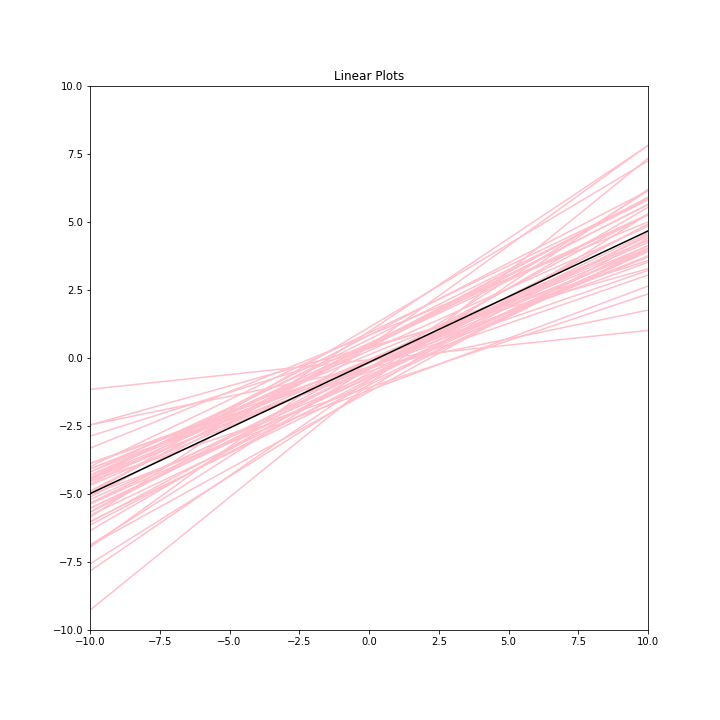
\includegraphics[scale=0.7]{q3_linear_v2.png}
            \caption{Linear Plots}
            \label{fig:linear_plots}
        \end{figure}
    \item[b.] Below are the quadratic plots. The average curve is depicted by the black colored line in the middle. As we can see in the figure, instead of being a quadratic function, the average curve is simply a linear function.
        \item[]
        \begin{figure}[H]
            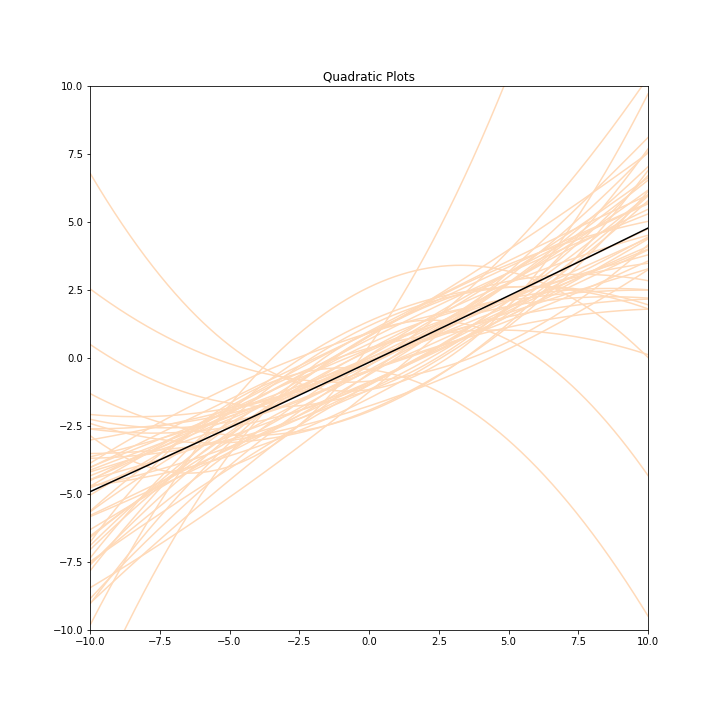
\includegraphics[scale=0.7]{q3_quadratic_v2.png}
            \caption{Quadratic Plots}
            \label{fig:quadratic_plots}
        \end{figure}
    \item[c.] Below are the cubic plots. The average curve is depicted by the black colored curve in the middle. We can see that, only for this regression, the average curve is not a linear function. It starts to look like a curve when x is greater than 6. This will be explained more in section d.
        \item[]
        \begin{figure}[H]
            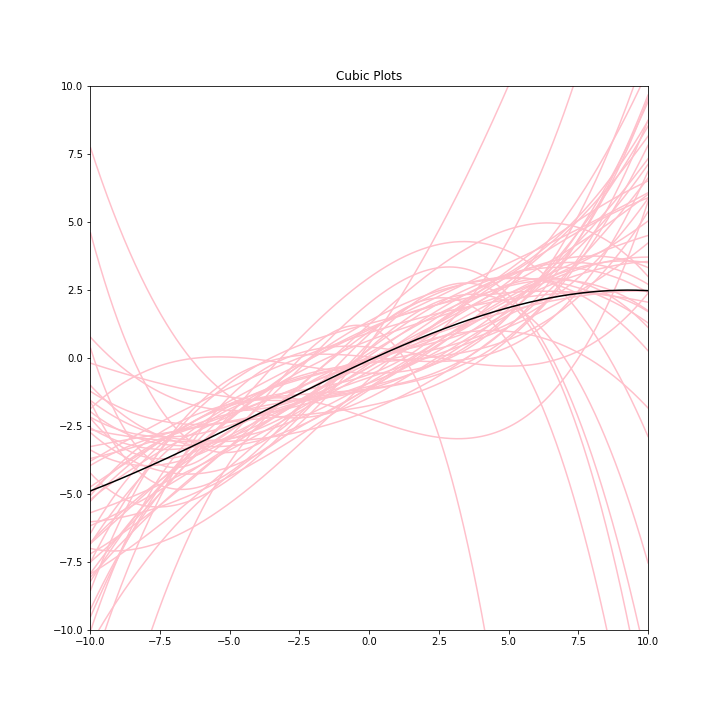
\includegraphics[scale=0.7]{q3_cubic_v2.png}
            \caption{Qubic Plots}
            \label{fig:cubic_plots}
        \end{figure}
    \item[d.] For linear regression using cubical feature map (section c), for $6\leq{x}\leq{10}$, this is because.
\end{itemize}
\newpage

\section*{Problem 4}
\begin{itemize}
    \item[a.]
\end{itemize}
\newpage

\section*{Problem 5}
\begin{itemize}
    \item[a.] The test risk of $\hat{f}$ is \boldsymbol{4.034974776250005}. The plot of outlier-ness is as below. The black dots are for the first 900 train data and the red dots are for the last 100 train data. The affine function that I got is $\boldsymbol{\hat{f}(x)= 1.065x + 0.2403}$.
    \item[]
        \begin{figure}[H]
            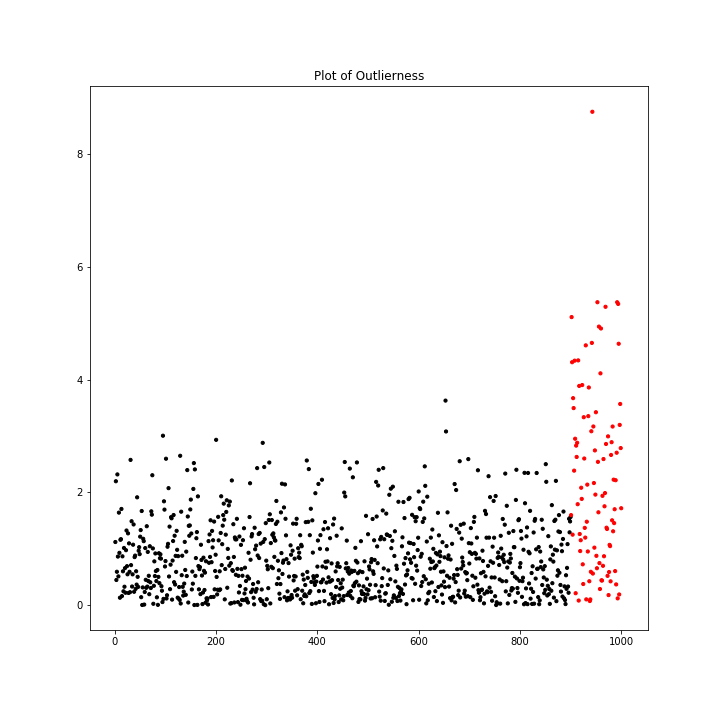
\includegraphics[scale=0.7]{q5_outlier_plot.png}
            \caption{Plot of Outlierness}
            \label{fig:plot_of_outi}
        \end{figure}
    \item[b.] Let's define the affine function $g(x)=mx+b$ and expand the risk function.
    $$\hat{R}_{Q_n}(g)=\frac{1}{2*900}\sum_{i=1}^{900}(g(x_i)-y_i)^2+\frac{1}{2*100}\sum_{i=901}^{1000}(g(x_i)-y_i)^2$$
    $$\hat{R}_{Q_n}(g)=\frac{1}{2*900}\sum_{i=1}^{900}(m(x_i)+b-y_i)^2+\frac{1}{2*100}\sum_{i=901}^{1000}(m(x_i)+b-y_i)^2$$

    For readability, let's expand our risk equation for $1\leq{i}\leq{900}$ first so that the equation won't be too long.
    $$\hat{R}_{Q_n}(g)_{{1..900}}=\frac{1}{2*900}\sum_{i=1}^{900}(m(x_i)+b-y_i)^2$$
    $$\hat{R}_{Q_n}(g)_{{1..900}}=\frac{1}{2*900}\sum_{i=1}^{900}(m^2{x_i}^2+2mx_ib+b^2-2mx_iy_i-2by_i+{y_i}^2)$$
    $$\hat{R}_{Q_n}(g)_{{1..900}}=\frac{1}{2*900}(m^2\sum_{i=1}^{900}{x_i}^2+2mb\sum_{i=1}^{900}x_i+b^2\sum_{i=1}^{900}1-2m\sum_{i=1}^{900}x_iy_i-2b\sum_{i=1}^{900}y_i+\sum_{i=1}^{900}{y_i}^2)$$

    We know that the sum of all elements is the same as the mean of all the elements multiplied by the number of elements. Let's define another term j in which $\overline{x_j}, \overline{y_j}, \overline{x_jy_j}, \overline{x_j^2}, \overline{y_j^2}$ respectively denotes the average of $x_i, y_i, x_iy_i, x_i^2, y_i^2$ for $1\leq{i}\leq{900}$. That gives us:
    $$\hat{R}_{Q_n}(g)_{{1..900}}=\frac{1}{2*900}(900m^2\overline{{x_j}^2}+2*900mb\overline{x_j}+900b^2-2*900m\overline{x_jy_j}-2*900b\overline{y_j}+900\overline{{y_j}^2})$$
    $$\hat{R}_{Q_n}(g)_{{1..900}}=\frac{1}{2}(m^2\overline{{x_j}^2}+2mb\overline{x_j}+b^2-2m\overline{x_jy_j}-2b\overline{y_j}+\overline{{y_j}^2})$$

    Using the very same steps, we can obtain a similar result for $901\leq{i}\leq{1000}$. By also defining another term, say k, in which $\overline{x_k}, \overline{y_k}, \overline{x_ky_k}, \overline{x_k^2}, \overline{y_k^2}$ respectively denotes the average of $x_k, y_k, x_ky_k, x_k^2, y_k^2$ for $901\leq{i}\leq{1000}$, the risk equation would be:
    $$\hat{R}_{Q_n}(g)_{{901..1000}}=\frac{1}{2}(m^2\overline{{x_k}^2}+2mb\overline{x_k}+b^2-2m\overline{x_ky_k}-2b\overline{y_k}+\overline{{y_k}^2})$$

    Finally, summing them would result in:
    $$\hat{R}_{Q_n}(g)=\frac{1}{2}(m^2(\overline{{x_j}^2}+\overline{{x_k}^2})+2mb(\overline{x_j}+\overline{x_k})+2b^2-2m(\overline{x_jy_j}+\overline{x_ky_k})-2b(\overline{y_j}+\overline{y_k})+(\overline{{y_j}^2}+\overline{{y_k}^2}))$$

    We then want to find $m$ and $b$ such that $\hat{R}_{Q_n}$ is minimum. We can do this by taking the first derivative against $m$ and against $b$ and respectively find $m$ and $b$ value that make each of them zero.

    $$\frac{d}{dm}(\hat{R}_{Q_n}(g))=0$$
    $$m(\overline{x_j^2}+\overline{x_k^2})+b(\overline{x_j}+\overline{x_k})-(\overline{x_jy_j}+\overline{x_ky_k})=0\:\:...\:(Eq. 1)$$

    $$\frac{d}{db}(\hat{R}_{Q_n}(g))=0$$
    $$m(\overline{x_j}+\overline{x_k})+2b-(\overline{y_j}+\overline{y_k})=0\:\:...\:(Eq. 2)$$

    We can eliminate $b$ by multiplying Equation 2 with $\overline{x_j}+\overline{x_k}$ and by multiplying Equation 1 by 2 and then subtract Equation 1 with Equation 2 (after the multiplications). In mathematical notation, $2*(Eq.\:1)-(\overline{x_j}+\overline{x_k})*(Eq.\:2)=0$.
    $$m(2(\overline{x_j^2}+\overline{x_k^2})-(\overline{x_j}+\overline{x_k})^2)-2(\overline{x_jy_j}+\overline{x_ky_k})+(\overline{x_j}+\overline{x_k})(\overline{y_j}+\overline{y_k})=0$$
    $$m=\frac{2(\overline{x_jy_j}+\overline{x_ky_k})-(\overline{x_j}+\overline{x_k})(\overline{y_j}+\overline{y_k})}{2(\overline{x_j^2}+\overline{x_k^2})-(\overline{x_j}+\overline{x_k})^2}$$

    We got our $m$. We can then substitute $m$ in Equation 2 to get our b.
    $$b=\frac{1}{2}((\overline{y_j}+\overline{y_k})-\frac{2(\overline{x_jy_j}+\overline{x_ky_k})-(\overline{x_j}+\overline{x_k})(\overline{y_j}+\overline{y_k})}{2(\overline{x_j^2}+\overline{x_k^2})-(\overline{x_j}+\overline{x_k})^2}(\overline{x_j}+\overline{x_k}))$$

    Finally, by calculating all the needed variables from each subpopulation and by using those two equations, the affine function that I got is $\boldsymbol{\hat{g}(x)= 1.1258x+ 0.8411}$.

    \item[c.] The test risk of $\hat{g}$ is \boldsymbol{3.642645831591768}, better than the test risk of $\hat{f}$.

    \item[d.] The test risks of each subpopulation of size 500 is as stated below in Table 1.
        \item[]
            \begin{table}[h!]
                \centering
                \begin{tabular}{||c c c||}
                    \hline
                    $\:$ & Test Subpopulation 1 & Test Subpopulation 2 \\ [0.5ex]
                    \hline\hline
                    $\hat{f}$  & 1.14655962195859 & 6.92338993054142\\
                    \hline
                    $\hat{g}$ & 1.8277141906456527 & 5.457577472537884\\
                    \hline
                \end{tabular}
                \caption{Subpopulation Test Risks Table}
                \label{table:1}
            \end{table}

    \item[e.] Test risk of $\boldsymbol{\hat{h}_1}$ in test subpopulation 1 is \boldsymbol{1.0840055002248241} and the test risk of $\boldsymbol{\hat{h}_2}$ in test subpopulation 2 is \boldsymbol{1.015860502522174}. As additional information, $\boldsymbol{\hat{h}_1=1.0031x+0.0526}$ and $\boldsymbol{\hat{h}_2=-0.9325x+9.7305}$.
\end{itemize}
\newpage

\end{document}

Let's define another term j in which $\overline{x_j}, \overline{y_j}, \overline{x_jy_j}, \overline{x_j^2}, \overline{y_j^2}$ respectively denotes the average of $x_i, y_i, x_iy_i, x_i^2, y_i^2$ for $1\leq{i}\leq{900}$. That gives us:
    $$\hat{R}_{Q_n}(g)_{{1..900}}=\frac{1}{2*900}(900m^2\overline{{x_j}^2}+2*900mb\overline{x_j}+900b^2-2*900m\overline{x_jy_j}-2*900b\overline{y_j}+900\overline{{y_j}^2})$$
    $$\hat{R}_{Q_n}(g)_{{1..900}}=\frac{1}{2}(m^2\overline{{x_j}^2}+2mb\overline{x_j}+b^2-2m\overline{x_jy_j}-2b\overline{y_j}+\overline{{y_j}^2})$$

    Using the very same steps, we can obtain a similar result for $901\leq{i}\leq{1000}$. By also defining another term, say k, in which $\overline{x_k}, \overline{y_k}, \overline{x_ky_k}, \overline{x_k^2}, \overline{y_k^2}$ respectively denotes the average of $x_k, y_k, x_ky_k, x_k^2, y_k^2$ for $901\leq{i}\leq{1000}$, the risk equation would be:
    $$\hat{R}_{Q_n}(g)_{{901..1000}}=\frac{1}{2}(m^2\overline{{x_j}^2}+2mb\overline{x_j}+b^2-2m\overline{x_jy_j}-2b\overline{y_j}+\overline{{y_j}^2})$$
